\documentclass{article}
\usepackage[framed]{seqcode}	% Also includes listings package

\usepackage{tabularx}
\usepackage{multirow}
\usepackage{makecell}

\usepackage{graphicx}
\usepackage{float}

\usepackage{booktabs}

\renewcommand{\cellalign}{tl}
\usepackage[bookmarks=true,ocgcolorlinks=true,plainpages=false, breaklinks=true, bookmarksopen=true, bookmarksnumbered=true]{hyperref}
\hypersetup{linkcolor=blue, citecolor=magenta,urlcolor=blue} % electronic
\hypersetup{colorlinks=true}
\hypersetup{
    pdftitle={Open file format for MR sequences},    % title
    pdfauthor={Kelvin Layton},                     % author
    pdfsubject={Specification for NMR and MRI sequences},                        % subject of the document
    pdfkeywords={Magnetic Resonance Imaging,spectroscopy,MRI,NMR,MR,open format,Pulseq}, % list of keywords
    }

%\def\myversion{1.01 }
\def\myversionmajor{1}
\def\myversionminor{4}
\def\myversionrevision{1}
\def\myversion{\myversionmajor.\myversionminor.\myversionrevision }
%\def\myversion{1.0.2 }




\date{}
\author{}


\lstset{% general command to set parameter(s)
%basicstyle=\small, % print whole listing small
% underlined bold black keywords
identifierstyle=, % nothing happens
%stringstyle=\ttfamily, % typewriter type for strings
showstringspaces=true,
%showlines=true,
%numbers=left,
belowskip=0em,
aboveskip=1em,
frame=single
} % no special string spaces


\definecolor{shadecolor}{gray}{0.96}

\newcommand{\superscript}[1]{\ensuremath{^{\textrm{#1}}}}


\usepackage{hyperref}



\begin{document}

\begin{titlepage}
\begin{centering}
\rule{\textwidth}{5pt}\vskip1cm
\Huge{Open file format for MR sequences \\}
\vspace{1cm}
\LARGE{Version \myversion (DRAFT)\\}
\vspace{1cm}
\large Maxim Zaitsev\\ Stefan Kroboth\\ Kelvin Layton\\ 
\vspace{1cm}
\large University Medical Centre Freiburg \\%
% \verb+kelvin.layton@uniklinik-freiburg.de+\\%
 \verb+maxim.zaitsev@uniklinik-freiburg.de+\\%
% \verb+stefan.kroboth@uniklinik-freiburg.de+\\%
 \vspace{1cm}
 This file specification is part of the Pulseq project:
 \vspace{0.5cm}
 \url{http://pulseq.github.io/}\\
 \href{http://pulseq.github.io/}{
\includegraphics[width=0.3\textwidth]{logo}}
 \vfill
\small This file format is licensed under the Creative Commons Attribution 4.0 International License. To view a copy of this license, visit \url{ http://creativecommons.org/licenses/by/4.0/ }\\
\rule{\textwidth}{5pt}
\end{centering}
\end{titlepage}

\newpage

\setlength\parindent{0pt}
\setlength{\parskip}{0.4\baselineskip}%

\tableofcontents

\setlength\parindent{0pt}
\setlength{\parskip}{\baselineskip}%

\newpage
\section*{Revision History}
\begin{tabular}{lll}
\toprule
Version & Date & Description \\
\midrule
1.0 & 26 Jun 2014 & Draft specification \\
1.01 & 11 Jun 2015 & Included draft of binary specification \\
1.1.0 & 11 Jul 2017 & Changed versioning scheme \\
1.2.0 & 06 Jul 2018 & \makecell{Events can now be delayed individually; \\ Delay events and other events overlap within blocks} \\
1.2.1 & 13 Dec 2018 & \makecell{Matlab code does not use zero-filling prior to the \\ actual RF shape to account for RF dead time and \\ uses delay instead. Interpreter code also does not \\ attempt to detect RF zero-filling.} \\
1.3.0 & 02 Jul 2019 & \makecell{Support for generic extensions: \\ added extensions column to the event table, which \\ references the new [extensions] section; \\ added support for one extension: \\ triggers (including two types: input and output).} 
\\
1.3.1 & 25 Sept 2020 & \makecell{Added support for the LABEL extension, updated figures. } 
\\
1.4.0 & 7 Jul 2021 & \makecell{Substantial revisions of the file format: \\ added required definitions; \\ we now explicitly specify sampling and raster alignment conventions; \\ flexible shape timing for arbitrary gradients and RF pulses; \\ explicit block duration; \\ removed [DELAYS]; \\ added uncompressed shape option; \\ added signature section. } 
\\
1.4.1 & 16 Feb 2023 & \makecell{New flags to the LABEL extension added; \\ TODO: update figures and examples. } \\
\bottomrule
\end{tabular}


\section{Introduction}
The purpose of this file format is to compactly represent a magnetic resonance (MR) sequence in an open and vendor independent manner. Sequences for both NMR spectroscopy and MRI can be represented. The format is intended for research and educational purposes and currently omits complex sequence features such as physiological triggering or logical coordinate-frame transformations. The format has been developed with the following \textbf{design goals}:
\begin{enumerate}
\item \textbf{Human-readable:} The basic sequence structure should be easily understood without processing.
\item \textbf{Easily parsed:} The format should be easy for a computer program to parse without the need for external libraries.
\item \textbf{Vendor independent:} The sequence format must not contain definitions specific to a particular hardware manufacturer.
\item \textbf{Compact:} The sequence must not contain redundant definitions. As such, re-use of existing definitions at different times is inherent in the sequence format.
\item \textbf{Low-level:} The format should be sufficiently low-level. This allows for maximum flexibility of sequence specifications and does not limit the high-level design tools.
\end{enumerate}

The first goal of human readability necessitates a text-file format. The file format is intended to describe a sequence that can be run on scanner hardware. Therefore, the second goal of machine readability ensures that the file can be read and interpreted without the use of external libraries that might be unavailable on different platforms. This prohibits the use of an existing markup language like XML, which are not straightforward to parse. Further, units  that are inherently hardware dependent have been avoided, such as `Volts' or `Tesla'. 


\subsection{Example}

Before defining the detailed specification, a simple example is presented to demonstrate the main structure of a sequence. Below is a simple FID experiment with RF pulse, delay and ADC readout. 
\lstinputlisting{../tests/fiddisp.seq}



\section{Specification}\label{sec:specification}

\subsection{Overall Description}

\begin{figure}[H]
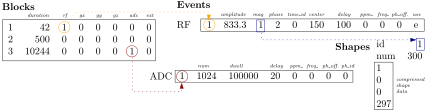
\includegraphics[width=\columnwidth]{block_diagram}
\caption{Visualisation of the hierarchical structure of the file format for an FID example. \label{fig:block_diagram}}
\end{figure}

The sequence description consists of a three-level hierarchical structure as demonstrated in Figure~\ref{fig:block_diagram}. This ensures the most compact representation, since repeating events (or shapes) are only declared once.
\begin{description}
\item[Blocks] At the top level the sequence is specified by a number of blocks. Each block refers to one or more event(s) to be executed simultaneously.
\item[Events] The definition of events are dependent on the type (e.g. gradient, ADC) but some types may refer to one or more basic shapes.
\item[Shapes] A shape is a compressed list of samples. The uncompressed samples can describe, for example, the RF pulse shape or an arbitrary gradient shape. The compression scheme is a type of run-length encoding.
\end{description}

Comments are specified by a line starting with a hash.
\begin{lstlisting}
# This is a comment
\end{lstlisting}

The numeric values are declared exactly as described below with storage defined by the value type. In general, \textbf{integer} types are stored as 64-bit unsigned integers while \textbf{floating-point} numbers are in the 64-bit IEEE 754 floating-point format. Exceptions are \verb.<id>. values, which are 32-bit integers. Shapes are stored as 32-bit short floats.

\subsection{Identification numbers}
A key idea of the hierarchical sequence structure is the use of ID numbers to refer to objects defined one level below in the hierarchy. For example, blocks contain the ID of one or more event(s). Likewise, events may contain the ID of one or more shape(s). Restrictions are placed on these IDs to ensure consistency:
\begin{itemize}
\item IDs must be positive integers.
\item The ID of each shape must be unique.
\item The ID of events within a single class must be unique. For example, an RF event and delay event may both use an ID of 1, since the events are of a different class. An exception is the \verb.[GRADIENTS]. and \verb.[TRAP]. events where the union of these sets must contain unique event IDs.
\item The ID of 0 for a time shape corresponds to the "default", meaning an incremental time sampling with the corresponding time raster.
\item There are no restrictions on the ordering of IDs, although sequential ordering is often implemented.
\item There are no restrictions on the first ID of an event class.
\end{itemize}

\subsection{Version}

The versioning scheme is $\langle$major$\rangle$.$\langle$minor$\rangle$.$\langle$revision$\rangle$.

\begin{lstlisting}[escapechar=\%]
[VERSION]
major %$\langle$%major%$\rangle$%
minor %$\langle$%minor%$\rangle$%
revision %$\langle$%revision%$\rangle$%
\end{lstlisting}

Providing the version of the standard is vital for sequence execution.
If this section is not provided, the interpreter sequence may either refuse execution or assume version 1.0.0. It is recommended to reject Pulseq files without \verb.[VERSION]. section.

\textbf{Example:}
\begin{lstlisting}[escapechar=\%]
[VERSION]
major %\myversionmajor%
minor %\myversionminor%
revision %\myversionrevision%
\end{lstlisting}

\subsection{Signature}

The Pulseq file may end with an optional section \verb.[SIGNATURE]. as in the example below:

\begin{lstlisting}[escapechar=\%]
[SIGNATURE]
# This is the hash of the Pulseq file, calculated right before 
# the [SIGNATURE] section was appended to the file
Type md5
Hash 237b85c2aa46ba98076359cde263d6ee
\end{lstlisting}

The signature is generated by hashing the readily exported file with a corresponding algorithm (in this example md5sum) and appending the \verb.[SIGNATURE]. section. The new line character preceding the keyword \verb.[SIGNATURE]. is part of the signature and needs to be stripped away for the signature verification. The \verb.[SIGNATURE]. section must contain two following fields along with any additional information in the format identical to that of \verb.[DEFINITIONS]. (see below). 

\begin{tabularx}{\textwidth}{llX}
\toprule
Tag & Type & Description\\
\midrule
\verb.Type. & string & ID of the hashing algorithm (e.g. md5, sha1 or sha256) \\
\verb.Hash. & string & Hash value produced by the hashing function in the hexadecimal format \\
\bottomrule
\end{tabularx}

\subsection{Definitions}

The sequence may contain general definitions indicated by the \verb.[DEFINITIONS]. keyword. Each definition is defined on a new line with the following format
\begin{lstlisting}
<key> <value>
\end{lstlisting}
This defines a list of user-specified key/value pairs.

\begin{tabularx}{\textwidth}{llXl}
\toprule
Tag & Type & Description & Units\\
\midrule
\verb.<key>. & text & Name of user definition & -- \\
\verb.<value>. & any & Value of definition & -- \\
\bottomrule
\end{tabularx}

The \verb.<value>. field is separated by a single space or tab character from \verb.<key>. and is terminated at the end of the line. Any (additional) white space at the beginning and at the end of \verb.<value>. is ignored.

\textbf{Example:}
\begin{lstlisting}
[DEFINITIONS]
AdcRasterTime 1e-07 
BlockDurationRaster 1e-05 
GradientRasterTime 1e-05 
RadiofrequencyRasterTime 1e-06 
FOV 0.256 0.256 0.004 
Name epi 
TE 0.005
TR 0.01
TotalDuration 0.04268 
\end{lstlisting}

Starting from the Pulseq format revision 1.4.0, the following definitions are reserved, some of which are optional, whereas the definitions labeled as \textbf{required} are compulsory.

\begin{tabularx}{\textwidth}{lXl}
\toprule
Definition & Description & Status\\
\midrule
\verb.GradientRasterTime. & Default raster time (dwell time) of the shaped gradient events, specified in seconds & required \\
\verb.RadiofrequencyRasterTime. & Default raster time (dwell time) of the radio-frequency pulse shapes, specified in seconds & required \\
\verb.AdcRasterTime. & The value defining the alignment of the ADC dwell times; ADC dwell time must be integer multiple of the specified AdcRasterTime; AdcRasterTime is specified in seconds & required \\
\verb.BlockDurationRaster. & The value defining the alignment of the block durations, specified in seconds; the physical block duration must be integer multiple of the specified BlockDurationRaster; Block duration in the \verb.[BLOCKS]. section are specified in the units of BlockDurationRaster  & required\\
\verb.Name. & Human-readable name of the sequence & optional \\
\verb.FOV. & Field of view specified in meters in x, y and z directions given as a space-separated list of numbers \\
\verb.TotalDuration. & Total duration of the sequence is seconds \\
\bottomrule
\end{tabularx}

It is important to note that all definitions that are not  \textbf{required} are optional and do not affect the basic sequence execution. Precise timing is given by the low-level specification of events. The definitions section may be used for arbitrary user-specific purposes, including attaching metadata or hardware-dependent parameters.

\subsection{Time raster, temporal alignment and shape sampling conventions}

Accurate timing is essential for NMR and MRI experiments. To guarantee 	
unambiguous time definition Pulseq operates at discrete time raster. Depending on the particular hardware implementation details different electronic components may have different clock resolutions and correspondingly different raster times. 

For understanding the time raster alignment it is important to differentiate between the \verb.edges. and \verb.centers. of the time raster steps. All blocks and events are aligned to the corresponding \verb.edges. of the time raster. Block duration is required to be multiple of \verb.BlockDurationRaster., therefore each block can only start and end at the \verb.edges. of the block duration raster. Gradient events may only start at time points which are multiple of \verb.GradientRasterTime.; for trapezoid events, ramp times and plateau duration may also only be equal to multiples of \verb.GradientRasterTime.. In contrast to that, any default sampling points (e.g. sampling points of arbitrary-shape gradients) are aligned to the \verb.centers. of the corresponding raster steps. The same convention applies to the default RF shape sampling and ADC sampling points. This means that the time of the n-th point on the RF pulse shape, gradient shape or ADC sampling point can be calculated as $t_n=t_{start} + \Delta t(0.5+n)$. We will eventually add some figures and diagrams to this section to explain this important concept.


\subsection{Blocks}

The section containing sequence blocks is declared with the \verb.[BLOCKS]. keyword. Each subsequence line declares a single block specified by a duration and a list of six event IDs. An ID of 0 indicates no event.
\begin{lstlisting}
<id> <duration> <rf> <gx> <gy> <gz> <adc> <ext>
\end{lstlisting}

Each non-zero value among the six tags represents the ID of the corresponding event.

\begin{tabularx}{\textwidth}{llX}
\toprule
Tag & Type & Description\\
\midrule
\verb.<id>. & integer & ID of the sequence block \\
\verb.<duration>. & integer & duration of the current block in units of \verb.BlockDurationRaster. \\
\verb.<rf>. & integer & ID of the RF event \\
\verb.<gx>. & integer & ID of the gradient event on the X channel \\
\verb.<gy>. & integer & ID of the gradient event on the Y channel \\
\verb.<gz>. & integer & ID of the gradient event on the Z channel \\
\verb.<adc>. & integer & ID of the ADC event \\
\verb.<ext>. & integer & ID of the extension table entry \\
\bottomrule
\end{tabularx}

\begin{minipage}{\textwidth}
The sequence must declare at least one block. Any non-zero number of blocks may be defined. The blocks are executed sequentially. The duration of each block is defined explicitly by the second field of the block description. No event comprising this block is allowed to last longer than the specified block duration. The interpreters must to throw an error, should they detect such condition. X, Y and Z refer to physical scanner gradient channels. Block duration may be zero, e.g. for blocks containing only extension events with zero durations such as data labels. A block with nonzero duration containing no nonzero event IDs is a delay block. Interpreters must gracefully ignore delay blocks of 0 duration. \\

\textbf{Example:}
\begin{lstlisting}
[BLOCKS]
   1   319   1   0   0   2    0    0
\end{lstlisting}
\end{minipage}

The block above is the first in the sequence which has a duration of 319*\verb.BlockDurationRaster. and contains an RF pulse with ID of 1 and a z-gradient pulse with ID of 2. The block has no X gradient, Y gradient or ADC events, indicated by zero IDs and also no extension is specified.

\subsection{Events}

Events are defined in sections, each starting with one the following keywords: \verb.[RF]., \verb.[GRADIENTS]., \verb.[TRAP]., \verb.[ADC]. or \verb.[EXTENSIONS].. Each event is specified on a single line and contains an ID followed by type-specific definition.

\subsubsection{RF}
The RF section is declared with the \verb.[RF]. keyword. Following this declaration, each RF event is specified by a single line containing seven numbers.
\begin{lstlisting}
<id> <amp> <mag_id> <phase_id> <time_id> <delay> <freq> <phase>
\end{lstlisting}

The specifiers are

\begin{tabularx}{\textwidth}{llXl}
\toprule
Tag & Type & Description & Units\\
\midrule
\verb.<id>. & integer & ID of the RF event & -- \\
\verb.<amp>. & float & Peak amplitude & Hz \\
\verb.<mag_id>. & integer & Shape ID for magnitude profile & -- \\
\verb.<phase_id>. & integer & Shape ID for phase profile & --\\
\verb.<time_id>. & integer & Shape ID for the time sampling points, specified in the units of \verb.RadiofrequencyRasterTime.; 0 means default time raster & -- \\
\verb.<delay>. & integer & Delay before starting the RF pulse & $\rm \mu s$\\
\verb.<freq>. & float & Frequency offset & Hz \\
\verb.<phase>. & float & Phase offset & rad \\
\bottomrule
\end{tabularx}

\begin{minipage}{\textwidth}
\textbf{Example:}
\begin{lstlisting}
[RF]
  1    2500  1   2  0  0  0.000  0.000
\end{lstlisting}
\end{minipage}

In the example above, the RF pulse has ID of 1, peak amplitude of 2500Hz. The magnitude and phase profiles are defined with the shapes of ID 1 and 2, respectively. The RF pulse does not have any frequency or phase offset or delay and uses the default time axis sampling with a dwell time of \verb.RadiofrequencyRasterTime..

\subsubsection{Gradients}
Gradient events are declared in two sections. Arbitrary gradients are in a section declared with the \verb.[GRADIENTS]. keyword. Each line in the section is an arbitrary gradient specified by four numbers,
\begin{lstlisting}
<id> <amp> <shape_id> <time_id> <delay>
\end{lstlisting}
Trapezoidal gradients are in a section declared with the \verb.[TRAP]. keyword. Each line in the section is a trapezoidal gradients specified by six numbers,
\begin{lstlisting}
<id> <amp> <rise> <flat> <fall> <delay>
\end{lstlisting}

The specifiers are

\begin{tabularx}{\textwidth}{llXl}
\toprule
Tag & Type & Description & Units\\
\midrule
\verb.<id>. & integer & ID of the gradient event & -- \\
\verb.<amp>. & float & Peak amplitude & Hz/m \\
\verb.<shape_id>. & integer & Shape ID for arbitrary gradient waveform & -- \\
\verb.<time_id>. & integer & Shape ID for the time sampling points, specified in the units of \verb.GradientRasterTime.; 0 means default time raster & -- \\
\verb.<rise>. & integer & Rise time of the trapezoid & $\rm \mu s$ \\
\verb.<flat>. & integer & Flat-top time of the trapezoid & $\rm \mu s$ \\
\verb.<fall>. & integer & Fall time of the trapezoid & $\rm \mu s$ \\
\verb.<delay>. & integer & Delay before starting the gradient event & $\rm \mu s$\\
\bottomrule
\end{tabularx}

The gradient ID must be unique across both arbitrary and trapezoid gradients. That is, a trapezoid gradient cannot have the same ID as an arbitrary gradient.


\begin{minipage}{\textwidth}
\textbf{Example:}
\begin{lstlisting}
[GRADIENTS]
  1    159154.9  3  4  0
[TRAP]
  2       25000    30  940  30  100
  3    20066.89    10  980  10  100
\end{lstlisting}
\end{minipage}

The example above contains two gradients: an arbitrary gradient with peak amplitude of approximately 159kHz/m and shape ID 3 and time shape ID 4 and two trapezoid gradients (IDs 2 and 3) with duration 1ms specified by amplitude, rise time, flat-top time and fall time.
Both gradients have a delay of 100$\rm \mu s$.

\subsubsection{ADC}
The ADC section is declared with the \verb.[ADC]. keyword. Each line in the section is an ADC event specified by six numbers,
\begin{lstlisting}
<id> <num> <dwell> <delay> <freq> <phase>
\end{lstlisting}

The specifiers are

\begin{tabularx}{\textwidth}{llXl}
\toprule
Tag & Type & Description & Units\\
\midrule
\verb.<id>. & integer & ID of the ADC event & -- \\
\verb.<num>. & integer & Number of samples & -- \\
\verb.<dwell>. & float & The ADC dwell time & $\rm n s$ \\
\verb.<delay>. & integer & Delay between start of block and first sample & $\rm \mu s$  \\
\verb.<freq>. & float & Frequency offset of ADC receiver & Hz \\
\verb.<phase>. & float & Phase offset of ADC receiver & rad \\
\bottomrule
\end{tabularx}

The duration of the ADC readout is given by the product of \verb.<num>. and \verb.<dwell>..

\begin{minipage}{\textwidth}
\textbf{Example:}
\begin{lstlisting}
[ADC]
  1    512  5000  0  0.000   0.000
\end{lstlisting}
\end{minipage}

The example above contains an ADC with 512 samples, and dwell time of 5000ns, and no frequency and phase offsets. The frequency and phase offset are used, for example, for RF spoiling or in-plane shifting of the FOV.

\subsubsection{Extensions}
Extensions concept allows for implementing additional features without requiring major revisions of the Pulseq format specification. Extensions can be defined in the design tool in a good hope that the particular interpreter will know how to handle it. The interpreter MUST detect unknown extensions and MAY chose to ignore them. It is recommended that the interpreter issues a warning in this case. 

The EXTENSIONS section is declared with the \verb.[EXTENSIONS]. keyword. Each line in the section is an extension table entry specified by four numbers,
\begin{lstlisting}
<id> <type> <ref> <next>
\end{lstlisting}

\begin{tabularx}{\textwidth}{llXl}
\toprule
Tag & Type & Description \\
\midrule
\verb.<id>. & integer & ID of the extension list entry \\
\verb.<type>. & integer & ID of the type of the extension \\
\verb.<ref>. & integer & ID of the extension object \\
\verb.<next>. & integer & ID of the next entry in the list \\
\bottomrule
\end{tabularx}

Extensions form zero-terminated single-linked list. Therefore event table \verb.[BLOCKS]. can reference a chain of extensions, which allows one to add more than one extension per block. \\

Extension list is followed by the actual specification of particular extensions. The specification has the following format:

\begin{lstlisting}
extension <STRING_ID> <type>
\end{lstlisting}

where 

\begin{tabularx}{\textwidth}{llXl}
\toprule
Tag & Type & Description \\
\midrule
\verb.extension. & keyword & Keyword specifying the beginning of the particular extension specification \\
\verb.<STRING_ID>. & integer & text ID of the present extension used by the interpreter to recognize the extension \\
\verb.<type>. & integer & ID of the type of the particular extension, referenced by the extension list \\
\bottomrule
\end{tabularx}

The interpreters MUST only use the \verb.STRING_ID. to recognize the extensions and do not count on particular value of the \verb.<type>. parameter. The latter is only valid within the single Pulseq file and MAY change from one file to another, or different unique type ID values may be used by different Pulseq export implementations.

\begin{minipage}{\textwidth}
\textbf{Example:}
\begin{lstlisting}
[EXTENSIONS]
1 1 1 0
2 1 2 0

extension TRIGGERS 1
1 2 1 0 2000
2 1 3 500 100
\end{lstlisting}
\end{minipage}

The example above contains a specification of the TRIGGERS extension, which is not a part of the core Pulseq format and MAY be subject to rapid changes between revisions. Current example above specifies one cardiac trigger (id=1 type=2 channel=1) and one digital output signal (id=2 type=1 channel=3) on the "external trigger" channel (Siemens-specific).

\textbf{Label Extension}

Starting from revision 1.3.1 both Matlab Pulseq toolbox and the Siemens interpreter sequence support LABEL extension. The extension is intended to provide a possibility for the pulse sequence to pass counters and flags over to the raw data object and in this way to communicate with the image reconstruction routines. \\ 

Two types of extensions are currently defined: LABELSET and LABELINC. The former allows one to set the counter or flag value, the latter can be used to increment the counter (not compatible with flags). The following counters are supported at the moment: 
LIN, PAR, SLC, SEG, REP, AVG, SET, ECO, PHS that can take any integer values and flags NAV, REV, SMS, PMC, NOPOS, NOROT, NOSLC that can be 0 or 1 corresponding to boolean 'false' and 'true' values. \\

At the start of the sequence all counters and flags are automatically initialized to zero. During the run-time sequence maintains current values of all counters and flags, which can be modified with LABELSET and LABELINC directives at any time in the sequence. Also zero-duration blocks containing only LABEL extension directives are allowed. The values of the counters have no immediate effect until the next ADC directive is executed. At the moment of the ADC event the values of the counters are recorded and in case of the Siemens interpreter are copied to the ADC Data Header. Prior to the pertinent ADC direction the values of the counters can take any arbitrary excursions, e.g. can be negative or exceed matrix dimensions temporarily. This has no negative effects. \\

In case the same block contains LABELSET, LABELINC and ADC directives the following priorities apply (independent of the order the events were submitted to the block e.g. in the Matlab toolbox): First all LABELSET directives are processed, followed by all LABELINC and only then the values of the counters are captured and passed over to the ADC directive.  

New experimental labels have been introduced in revision 1.4.1. These include \verb.PMC., \verb.NOROT., \verb.NOPOS., \verb.NOSLC. and \verb.ONCE. flags (the latter explained further below). 

The meaning of the flags \verb.PMC., \verb.NOROT., \verb.NOPOS. and \verb.NOSLC. is as follows:

\begin{tabularx}{\textwidth}{llXl}
\toprule
ID & Type & Description\\
\midrule
\verb.PMC. & flag & Defines whether prospective motion correction (PMC) may be applied to the current block \\
\verb.NOROT. & flag & Instructs the interpreter to ignore translation components of the FOV positioning applied through the UI on the scanner or by the PMC processing (EXPERIMENTAL) \\
\verb.NOPOS. & flag & Instructs the interpreter to ignore translation components of the FOV positioning applied through the UI on the scanner or by the PMC processing (EXPERIMENTAL) \\
\verb.NOSLC. & flag & Instructs the interpreter to ignore FOV / gradient scaling parameters applied through the UI on the scanner (EXPERIMENTAL) \\
\bottomrule
\end{tabularx}

Additionally, there is a three-state flag \verb.ONCE., that is intended to control the execution flow for sequences with repetitions. It allows to implement dummy scans, warm-up sub-sequences, calibration scans or closing-up sub-sequences. The flag instructs the interpreter to alter the sequence when executing multiple repeats as follows: blocks with ONCE=0 are executed on every repetition; ONCE=1 marks the blocks that are only executed in the first repetition; blocks with ONCE=2 (or any other number) are only executed in the last repetition. When number of repetitions is equal to 1 no changes are applied.

\subsection{Shapes}

The shape section is declared with the \verb.[SHAPES]. keyword. Each shape is then declared with a header followed by a list of samples values (one per line). The end of the shape definition is declared with a blank line. Pulseq export software may opt for storing \textbf{uncompressed} shapes, e.g. to avoid rounding errors during compression/decompression or to save space for shapes that cannot be effectively compressed. The reading routines must interpret the shape as \textbf{uncompressed} if the number of samples in the stored shape is equal to \verb.Num_Uncompressed.. Therefore the saving routine must save the shape in uncompressed format if the result of compression has the same length as the original shape.

\begin{lstlisting}
Shape_ID <id>
Num_Uncompressed <num>
<sample_1>
<sample_2>
...
\end{lstlisting}

The specifiers are

\begin{tabularx}{\textwidth}{llXl}
\toprule
Tag & Type & Description & Units\\
\midrule
\verb.<id>. & integer & ID of the shape & -- \\
\verb.<num>. & integer & Number of samples of the uncompressed shape & -- \\
\verb.<sample_.$n$\verb.>. & integer & The $n^{\rm th}$ sample of the compressed shape  & -- \\
\bottomrule
\end{tabularx}

When used as amplitude shapes for gradient or RF objects, the decompressed samples must be in the normalised range of [-1, 1] (e.g. the absolute value of the shape must be normalized to the range of [0 1]). Since the purpose of this section is to define the basic shape of a gradient or RF pulse, the amplitude information is defined in the events section. This allows the same shape to be used with different amplitudes, without repeated definitions.

The number of points after decompressing all samples defined in a shape must equal the number declared in \verb.<Num_Uncompressed>..

\subsubsection{Compression}

Storing every sample of the shape would lead to very large sequence descriptions. Suppose a sequence contains a block RF pulse for 4ms and a sinusoidally-ramped constant gradient for 100ms. Assuming sampling times of $1{\rm \mu s}$ and $10{\rm \mu s}$ for the RF and gradients, respectively, $14000$ samples would be required. Instead, the shapes are compressed by \textbf{encoding the derivative in a run-length compressed} format. 

\textbf{Example 1: } A shape consisting of a ramp-up, constant and ramp-down is encoded as follows
\vspace{-1em}
\begin{center}
\begin{tabular}{rrrrr}
\toprule
Shape & & Step 1 (derivative) && Step 2 (compression) \\
\midrule
0.0 && 0.0 && 0 \\
0.1 && 0.1 && 0.1 \\
0.25&& 0.15&& 0.15 \\
0.5 && 0.25&& 0.25 \\
1.0 && 0.5 && 0.5 \\
1.0 && 0.0 && 0.0 \\
1.0 & $\rightarrow$& 0.0 & $\rightarrow$ & 0.0 \\
1.0 && 0.0 && 4 \\
1.0 && 0.0 && -0.25 \\
1.0 && 0.0 && -0.25 \\
1.0 && 0.0 && 2 \\
0.75&& -0.25 \\
0.5 && -0.25 \\
0.25&& -0.25 \\
0.0 && -0.25 \\
\bottomrule
\end{tabular}
\end{center}

\textbf{Example 2: } A shape with 100 zeros values
\vspace{-1em}
\begin{center}
\begin{tabular}{rrrrr}
\toprule
Shape & & Step 1 (derivative) && Step 2 (compression) \\
\midrule
0.0 && 0.0 && 0 \\
0.0 & $\rightarrow$ & 0.0 & $\rightarrow$ & 0 \\
$\cdots$ &  & $\cdots$ &  & 98 \\
0.0 && 0.0 &&  \\
\bottomrule
\end{tabular}
\end{center}

\textbf{Example 3: } A shape with a constant value of 1.0 for 100 samples
\vspace{-1em}
\begin{center}
\begin{tabular}{rrrrr}
\toprule
Shape & & Step 1 (derivative) && Step 2 (compression) \\
\midrule
1.0 && 1.0 && 1.0 \\
1.0 & $\rightarrow$ & 0.0 & $\rightarrow$ & 0 \\
$\cdots$ &  & $\cdots$  &  & 0 \\
1.0 && 0.0 &&  97 \\
\bottomrule
\end{tabular}
\end{center}

\section{Binary files}
 \textbf{Binary Pulseq format is not widely accepted and is poorly supported. This section is out-of-date.} The specification described in Section~\ref{sec:specification} can be implemented as a binary file. The same general principles apply with specific modifications outlined here. The basic structure of a binary \emph{pulseq} file is depicted below,
\texttt{
\begin{center}
\begin{tabular}{|c|c|c|c|c|c|c|c|l}
\hline
0x01 & p & u & l & s & e & q & 0x02 \\
\hline
%\multicolumn{8}{|c|}{0x0000000000000001} \\
\multicolumn{8}{|c|}{version major} \\
\hline
%\multicolumn{8}{|c|}{0x0000000000000001} \\
\multicolumn{8}{|c|}{version minor} \\
\hline
%\multicolumn{8}{|c|}{0x0000000000000000} \\
\multicolumn{8}{|c|}{version revision} \\
\hline
\multicolumn{8}{|c|}{section code} \\
\hline
\multicolumn{8}{|c|}{number of events} \\
\hline
\multicolumn{8}{|c|}{\multirow{2}{*}{data}} \\
\multicolumn{8}{|c|}{}\\
\hline
\multicolumn{8}{|c|}{section code} \\
\hline
\multicolumn{8}{|c|}{number of events} \\
\hline
\multicolumn{8}{|c|}{\multirow{2}{*}{data}} \\
\multicolumn{8}{|c|}{}\\
\hline
\multicolumn{8}{|c|}{$\cdots$}\\
\hline
\end{tabular}
\end{center}
}

\subsection{File and section codes}

A binary \textit{Pulseq} file begins with the 64 bit code \verb.0x0170756C73657102. (the characters \verb.pulseq. enclosed by \verb.0x01. and \verb.0x02.)  followed by three integers describing the file version (major, minor, revision). The remaining file is made up of multiple sections each with an integer section code followed by section-specific storage. The section codes corresponding to text file tags are

\begin{center}
\begin{tabular}{ll}
\toprule
Section & Section code \\
\midrule
\verb.[DEFINITIONS]. & \verb.0xFFFFFFFF 0x00000001. \\
\verb.[BLOCKS]. & \verb.0xFFFFFFFF 0x00000002. \\
\verb.[RF]. & \verb.0xFFFFFFFF 0x00000003. \\
\verb.[GRADIENTS]. & \verb.0xFFFFFFFF 0x00000004. \\
\verb.[TRAP]. & \verb.0xFFFFFFFF 0x00000005. \\
\verb.[ADC]. & \verb.0xFFFFFFFF 0x00000006. \\
\verb.[DELAYS]. & \verb.0xFFFFFFFF 0x00000007. \\
\verb.[SHAPES]. & \verb.0xFFFFFFFF 0x00000008. \\
\bottomrule
\end{tabular}
\end{center}

\section{Source code}
This specification is distributed with source code for reading and writing the sequences file format described here. MATLAB code is provided for detailed sequence generation, visualisation, as well as reading and writing sequence files. A C++ class and example program is also provided for reading sequence files. Detailed documentation and latest updates of this code are available here: \url{http://pulseq.github.io/}.

\newpage
\section{Examples}

\subsection{Free induction decay}

\lstinputlisting{../tests/fiddisp.seq}

\subsection{Point-resolved spectroscopy (PRESS)}

\lstinputlisting{../tests/pressdisp.seq}

\subsection{Gradient echo}

\lstinputlisting{../tests/gredisp.seq}


\end{document}
\grid
\grid
\grid
